\documentclass[5p,times]{elsarticle}
\usepackage[utf8]{inputenc}
\usepackage[spanish]{babel}
\usepackage{amsmath}
\usepackage{amsfonts}
\usepackage{amssymb}
\usepackage{graphicx}
\usepackage{url}
\usepackage{subcaption}
 
\usepackage{etoolbox}


\usepackage{float}


\begin{document}
\patchcmd{\abstract}{Abstract}{Resumen}{}{}
\begin{frontmatter}

\title{Análisis de datos de un concurso de cine}
\author{L.A. Gutierrez-Rodriguez}
\address{Posgrado de Ingeniería en Sistemas,\\ Facultad de Ingeniería Mecánica y Eléctrica,\\ Universidad Autónoma de Nuevo León}
\ead{luis.gutierrezrd@uanl.edu.mx}

\begin{abstract}
Contamos con los registros de un concurso de cine, cuyos filmes han sido grabados con dispositivos smartphone. Se busca identificar el alcance del certamen, ayudar a definir las mejores técnicas de difusión, caracterizar las categorías para equilibrar la cantidad de participantes, mejorar la forma en que se registraron los participantes y pronosticar la participación de los próximos años. La información se encuentra almacenada en cinco documentos de hoja de cálculo. Cada documento cuenta con los registros del concurso de cada año, del 2015 al 2018. Cuatro de ellos son del festival con sede en Colombia y el último del primer festival en México.

Se utiliza el lenguaje de programación Python y las librerías Numpy, Pandas, Scipy y MatPlotLib para realizar análisis estadístico sobre los datos y poder graficar los resultados. Se aplican modelos de regresión lineal y múltiple. Se analiza la varianza y las componentes principales de los datos. Se pronostica la cantidad de participantes de futuros años. Se implementa la librería SKLearn para clasificar y agrupar los datos. Se realiza análisis de texto de las sinopsis e imágenes de los vídeos ganadores. Al aplicar técnicas de estadística descriptiva se puede determinar que la mayoría de extranjeros que participan en el concurso son de México. 



\end{abstract}

\end{frontmatter}

\renewcommand{\abstractname}{Resumen}

\section*{Introducción}
En la actualidad contamos con una cantidad inmensa de datos debido a que almacenamos toda clase de información. Se busca darle un sentido útil a estos datos para poder comprenderlos. La ciencia de datos es el estudio de la extracción generalizable de conocimiento a partir de datos \cite{dhar2012data}. En este trabajo se busca aplicar la ciencia de datos ayudar en la toma de decisiones de dónde y cuándo se deben organizar los eventos, la mejor forma de organizar las categorías y en que otros países se puede expandir el festival. 

Se sabe que la mayoría de los concursantes son de regiones cercanas a la capital de Colombia, que estos concursantes usan smartphones para grabar sus vídeos, que proporcionan una sinopsis, y cada participante ubica su filme en un género. Además, no se tiene identificación de los participantes, y por esto no se puede trazar su participación a lo largo de los festivales.

En antecedentes hablaremos de todo lo relacionado con el festival de cine. En la literatura relacionada, se vera que problemas ya han sido tratados y como la obtención de información ayudó a la toma de decisiones. Además, se tratan temas que están relacionadas con el tipo de información que buscamos. En la metodología aplicada se mencionan las hipótesis que probamos sobre los datos y las herramientas utilizadas. En la sección de los resultados, se puede observar cómo se comportaron los datos con los análisis que probamos. Y en conclusión determinamos el sentido de nuestras hipótesis.

\section*{Antecedentes}
SmartFilms \cite{smartfilms} se ha convertido en el festival de cine más importante del momento en Colombia, gracias a los diferentes escenarios que les permiten a los participantes exhibir todo tipo de contenidos, usando los valores y conceptos de las marcas patrocinadoras de las diferentes categorías por medio del storytelling, product placement y branded content, de esta manera, marcar un nuevo camino hacia el crecimiento de las industrias, utilizando las empresas privadas como aliado en la producción cinematográfica.

Los participantes deben realizar un cortometraje de máximo cinco minutos, incluyendo créditos y este debe ser grabado en su totalidad con un celular o dispositivo móvil, adjuntar un making of (detrás de cámaras), adjuntar cartel de propaganda y enviar el cortometraje antes del cierre de la convocatoria.

El festival es anual. En cada proceso se realizan actividades pedagógicas y de activación para incentivar a las personas a que participen y fomenten la industria cinematográfica


\section*{Literatura relacionada}
A través del tiempo, el cine ha sido considerado el séptimo arte, la octava maravilla y por ello se han creado certámenes para apreciar el trabajo que conlleva realizar un film. El certamen más importante en el mundo del cine son los premios Oscar. Depende de la academia determinar cual film es ganador de ciertas categorías como iluminación, guión, director, actores, entre otros. Las tecnologías de la información son un rubro tan amplio que se extiende al cine. Se puede analizar la composición de imagen de un film no solo con el ojo de un experto, si no también con visión computacional. En \cite{oscars2013} se hizo un análisis predictivo y se buscaba determinar quienes serían los ganadores de las diversas categorías. Esta aplicación también ilustró cómo la Ciencia de Datos podría implementarse en las industrias de medios y entretenimiento.

En \cite{movie2015} se aplicó la minería de datos, minería de textos y análisis de redes sociales para aprender a analizar los datos de las películas. Se buscó una relación entre la información obtenida del análisis y la cantidad de estrellas otorgadas por el publico en la IMDB. Además compararon lo aprendido con datos reales obtenidos de una película Francesa. En \cite{inbook} se examinó el papel de los mercados de predicción en la evaluación de la probabilidad de que una película nominada reciba un premio de la Academia.

\section*{Metodología}
En esta sección veremos la información particular de los datos, y que herramientas utilizamos y con que fin. Se aplicó un proceso de limpieza de datos ya que estos presentaban espacios vacíos, errores de tipo de dato o se encontraban formas en las que se llenó un campo, siendo varias de ellas diferentes representaciones de la misma información. Finalmente, de acuerdo a que hipótesis se estaba probando, se seleccionaba solo algunos campos de los registros.


\subsection*{Datos}
Contamos con cinco documentos en formato de hoja de cálculo, los cuales son los registros al festival de cine. Estos datos representan los registros desde el año 2015 al 2018.


\subsection*{Herramientas}
Utilizamos las librerías Numpy \cite{numpy} y Pandas \cite{pandas} para la captura y almacenamiento de los datos limpios y poder trabajar con ellos.

Importamos la librería Scipy \cite{scipy} para poder realizar análisis estadísticos y MatPlotLib \cite{matplotlib} para graficar los resultados.

Se implementó SKLearn \cite{sklearn} para realizar clasificaciones y agrupamientos de los datos en base a su comportamiento.


\section*{Resultados}
Se graficaron los datos para ver si se podía concluir algo sobre éstos. Después se seleccionaron los participantes extranjeros de todos los cuatro años, y se ordenaron por el país de procedencia.

\subsection*{Categorizaciones}

Como se tienen muchas cadenas de texto en nuestros datos, es importante hacer categorizaciones ya que se hacen conteos de la información que se tiene disponible y así poder hacer cálculos estadísticos. Se aplica una categorización por país, pero se removieron los datos que involucran a México y Colombia que son los países anfitriones del concurso y por ende son los que sesgan la información, entonces esta información será relevante a los países extranjeros que participan. 


\subsubsection*{Regresión Lineal Simple}
La regresión lineal simple es un modelo de regresión lineal con una sola variable explicativa. Es decir, se trata de puntos de muestra bidimensionales con una variable independiente y una variable dependiente y encuentra una función lineal (una línea recta no vertical) que, con la misma precisión que posible, predice los valores de las variables dependientes en función de las variables independientes. El adjetivo simple se refiere al hecho de que la variable de resultado está relacionada con un solo predictor.

Con estas categorías se pudo buscar Modelos lineales y regresión múltiple.

\begin{figure}[H]
\centering
\begin{subfigure}[t]{0.2375\textwidth}
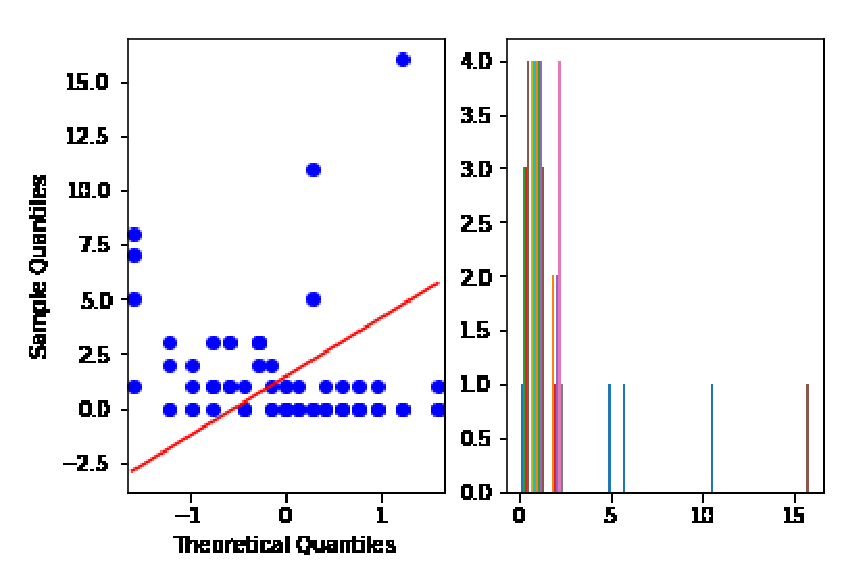
\includegraphics[width=\textwidth]{01}
\end{subfigure}
\hfill
\begin{subfigure}[t]{0.2375\textwidth}
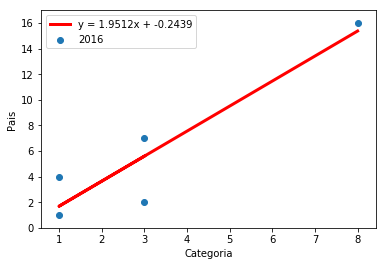
\includegraphics[width=\textwidth]{02}
\end{subfigure}
\vskip\baselineskip
\begin{subfigure}[b]{0.237\textwidth}
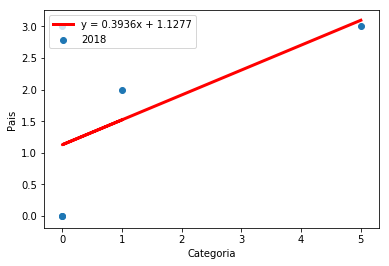
\includegraphics[width=\textwidth]{03}
\end{subfigure}
\hfill
\begin{subfigure}[b]{0.237\textwidth}
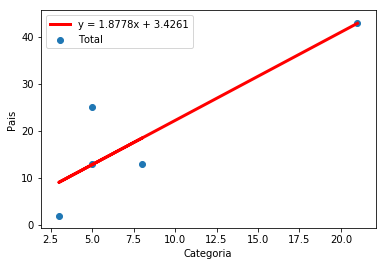
\includegraphics[width=\textwidth]{04}
\end{subfigure}
\caption{Modelos de regresion lineal}\label{fig:MRL}
\end{figure}


En la Figura \ref{fig:MRL} se observa como las rectas no quedaron significativas. En la Figura \ref{fig:MRLDist} se muestran las distribuciones de participantes por año.

\begin{figure}[H]
\centering
\begin{subfigure}[b]{0.2375\textwidth}
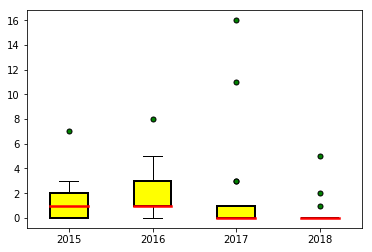
\includegraphics[width=\textwidth]{05}
\end{subfigure}
\hfill
\begin{subfigure}[b]{0.2375\textwidth}
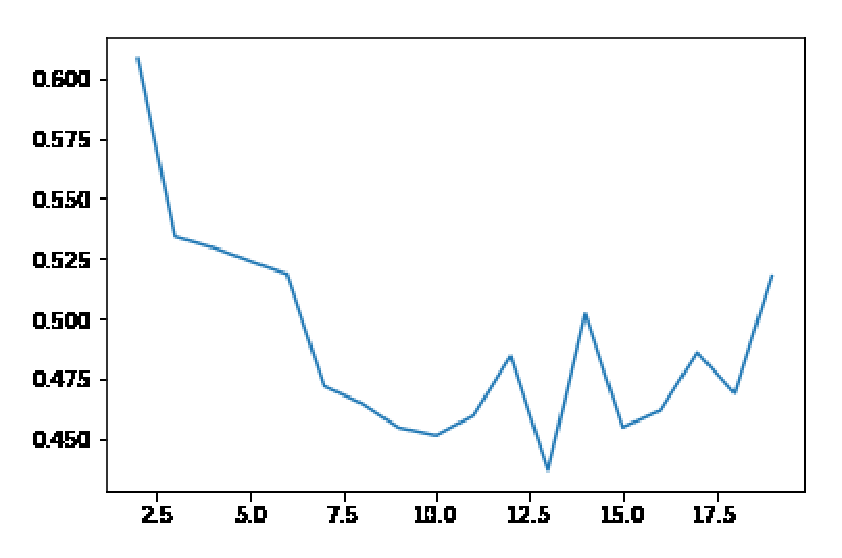
\includegraphics[width=\textwidth]{06}
\end{subfigure}
\caption{Distribución de participantes por año}\label{fig:MRLDist}
\end{figure}

Primero se probó la regresión de los datos por país de procedencia y por categoría de participación. Después se hizo un gráfico de bigote para entender la distribución de los datos.


\subsubsection*{Regresión Lineal Múltiple}

La regresión lineal permite trabajar con una variable a nivel de intervalo o razón. De la misma manera, es posible analizar la relación entre dos o más variables a través de ecuaciones, lo que se denomina regresión múltiple o regresión lineal múltiple. Constantemente en la práctica de la investigación estadística, se encuentran variables que de alguna manera están relacionadas entre sí, por lo que es posible que una de las variables puedan relacionarse matemáticamente en función de otra u otras variables. 

Los mínimos cuadrados ordinarios (OLS por sus siglas en ingles) es un método para encontrar los parámetros poblacionales en un modelo de regresión lineal. Este método minimiza la suma de las distancias verticales entre las respuestas observadas en la muestra y las respuestas del modelo. El parámetro resultante puede expresarse a través de una fórmula sencilla, especialmente en el caso de un único regresionador. 

En el Anexo A \ref{AnexoA}, se puede observar la prueba OLS que se le hizo a los parámetros. En esa prueba quedaron varios factores como No significativos, por eso se realiza una gráfica de dispersión de los datos para comprender su naturaleza, como se puede ver en la Figura \ref{fig:MRLM}. 


\begin{figure}[H]
\centering
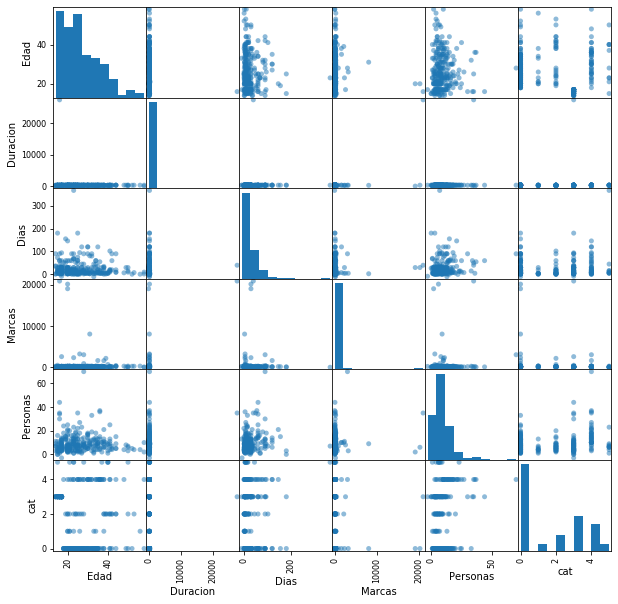
\includegraphics[width=0.35\textwidth]{09}
\caption{Modelos de regresion lineal múltiples}\label{fig:MRLM}
\end{figure}

Se hizo una regresión lineal múltiple entre los años de participación, para saber si existía correlación.


\subsection*{Aprendizaje Maquina}
También se usa la librería \textit{sklearn} para ver si las clasificaciones de las categorías ayudaban a entrenar a una red neuronal para que cuando se le entregaran otro conjunto de datos los clasificara correctamente.

Posteriormente, seguimos utilizando la librería para aplicar algoritmos de agrupamiento, para que los datos se ordenaran de acuerdo a sus propias características.

\subsubsection*{Algoritmo K-Means}

Este algoritmo \cite{hartigan1979algorithm} agrupa los datos al tratar de separar muestras en n grupos de igual varianza, minimizando un criterio conocido como la inercia o la suma de cuadrados dentro del grupo. Este algoritmo requiere que se especifique la cantidad de grupos. Se adapta bien a un gran número de muestras y se ha utilizado en una amplia gama de áreas de aplicación en muchos campos diferentes. En la Figura \ref{fig:MachineLearningG} en los incisos (a) se puede observar como se realizaron las $K$-medias, en el (b) se grafica el comportamiento de la precision de la clasificación al variar la $k$.


\begin{figure}[H]
\centering
\begin{subfigure}[t]{0.2375\textwidth}
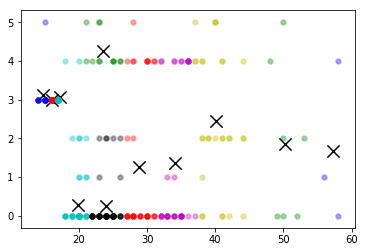
\includegraphics[width=\textwidth]{15}
\caption{}
\end{subfigure}
\hfill
\begin{subfigure}[t]{0.2375\textwidth}
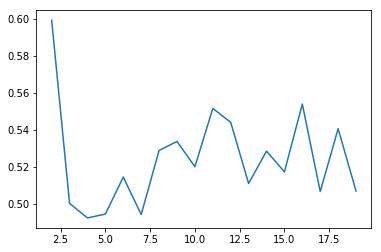
\includegraphics[width=\textwidth]{16}
\caption{}
\end{subfigure}
\hfill
\begin{subfigure}[t]{0.2375\textwidth}
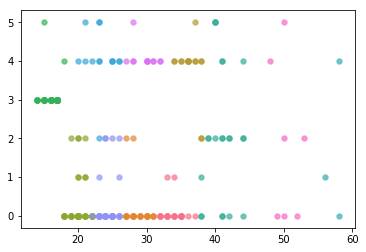
\includegraphics[width=\textwidth]{17}
\caption{}
\end{subfigure}\caption{Resultados de los métodos de aprendizaje maquina}\label{fig:MachineLearningG}
\end{figure}



Al aplicar el algoritmo de $K$-medias, el valor de $K$ usado fue dos. También evaluó cambiar el valor de $K$, y se obtuvo la siguiente gráfica.

\subsubsection*{Algoritmo Propagación de Afinidad}

Este algoritmo crea clústeres \cite{wang2008adaptive} enviando mensajes entre pares de muestras hasta la convergencia. Luego se describe un conjunto de datos utilizando un pequeño número de ejemplares, que se identifican como los más representativos de otras muestras. Los mensajes enviados entre pares representan la idoneidad para que una muestra sea el ejemplar de la otra, que se actualiza en respuesta a los valores de otros pares. Esta actualización ocurre de manera iterativa hasta la convergencia, momento en el que se eligen los ejemplares finales y, por lo tanto, se proporciona la agrupación final. En la Figura \ref{fig:MachineLearningG} en el inciso (c), se muestra como el Algoritmo determinó que también deberían ser once grupos, pero diferentes al de $K$-medias.


Se aplica el algoritmo Propagación de Afinidad sobre los mismos datos que el $K$-medias, donde también se dividió en dos grupos, pero la división de esos grupos se movió a mayor edad. En la Figura \ref{fig:MachineLearningR} se pueden ver las precisiones obtenidas en cada método probado sobre el mismo conjunto de datos. En el Anexo B \ref{AnexoB} se pueden ver las clasificaciones que hicieron los métodos. 


\begin{figure}[H]
\centering
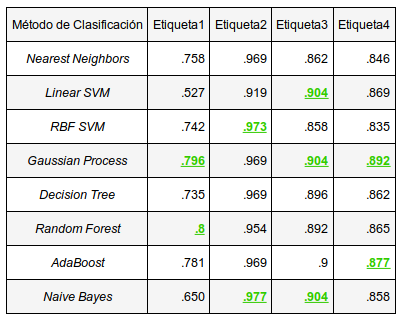
\includegraphics[width=0.3\textwidth]{14}
\caption{Resultados de los métodos de aprendizaje maquina}\label{fig:MachineLearningR}
\end{figure}


\section*{NLTK}

El kit de herramientas de lenguaje natural, o más comúnmente NLTK, es un conjunto de bibliotecas y programas para el procesamiento del lenguaje natural (PLN) simbólico y estadísticos para el lenguaje de programación Python. NLTK incluye demostraciones gráficas y datos de muestra.

Al usar NLTK para hacer análisis de texto, se obtuvo que en las sinopsis de los filmes cuentan con palabras que son muy frecuentemente usadas. Al hacer un mosaico con estas palabras como se ve en la Figura \ref{fig:NLTK}.

\begin{figure}[H]
\centering
\begin{subfigure}[t]{0.2375\textwidth}
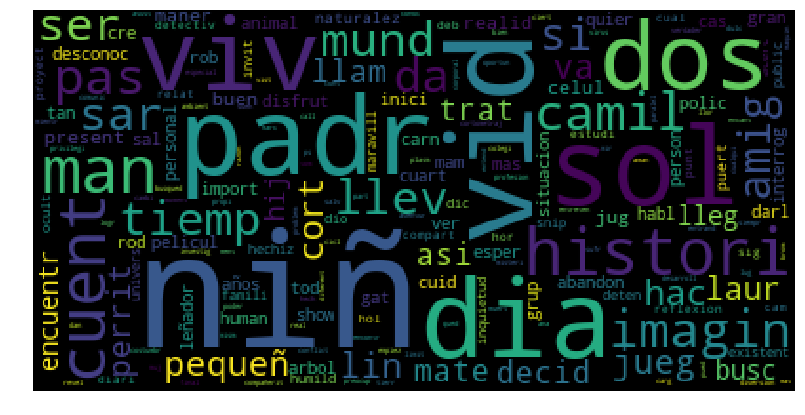
\includegraphics[width=\textwidth]{18}
\caption{}
\end{subfigure}
\hfill
\begin{subfigure}[t]{0.2375\textwidth}
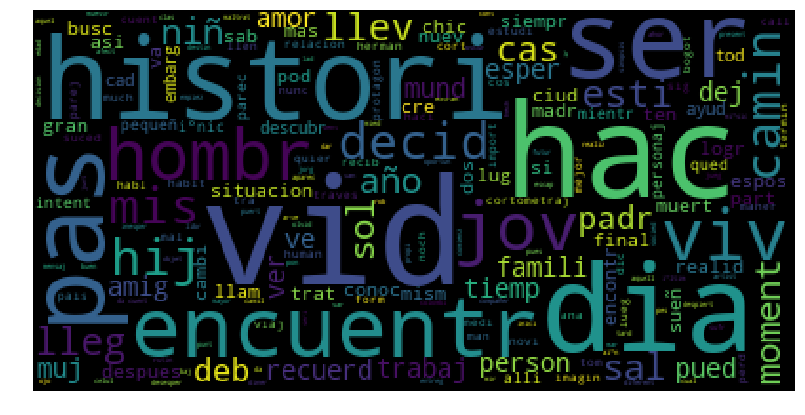
\includegraphics[width=\textwidth]{19}
\caption{}
\end{subfigure}
\vskip\baselineskip
\begin{subfigure}[t]{0.2375\textwidth}
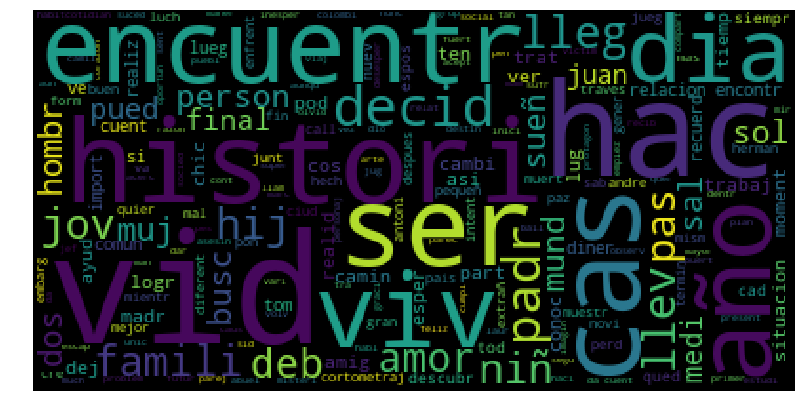
\includegraphics[width=\textwidth]{20}
\caption{}
\end{subfigure}
\hfill
\begin{subfigure}[t]{0.2375\textwidth}
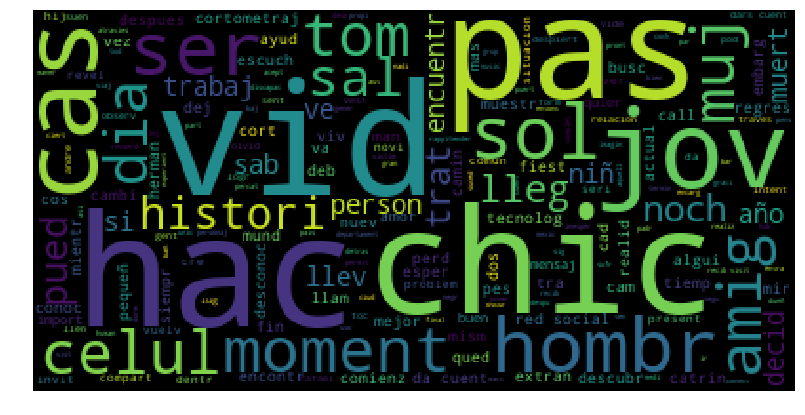
\includegraphics[width=\textwidth]{21}
\caption{}
\end{subfigure}
\caption{Mosaicos NLTK}\label{fig:NLTK}
\end{figure}



\section*{Análisis de Imágenes}

Se realiza un análisis de imágenes de los filmes ganadores de cada categoría. Se utilizó YouTube para obtener los vídeos, y OpenCV para poder hacer el procesamiento.

\subsection*{OpenCV}

OpenCV es una biblioteca libre de visión artificial originalmente desarrollada por Intel. Se ha utilizado en infinidad de aplicaciones. Desde sistemas de seguridad con detección de movimiento, hasta aplicaciones de control de procesos donde se requiere reconocimiento de objetos.


\begin{figure}[H]
\centering
\begin{subfigure}[t]{0.5\textwidth}
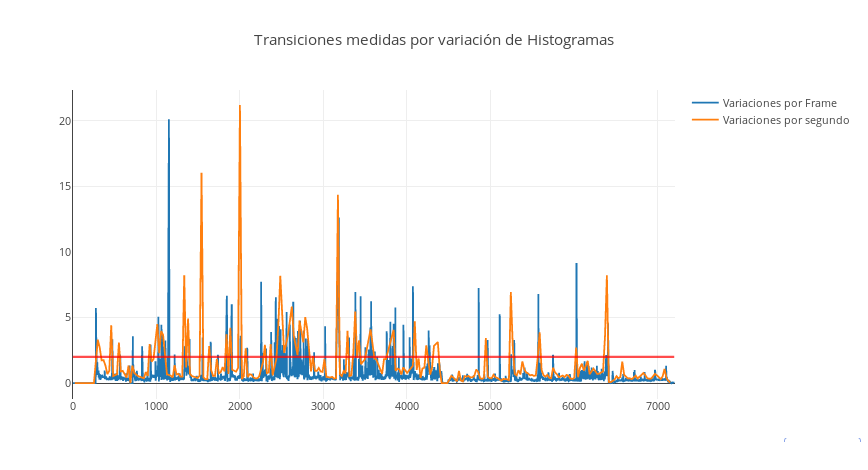
\includegraphics[width=\textwidth]{22}
\caption{}
\end{subfigure}
\hfill
\begin{subfigure}[t]{0.5\textwidth}
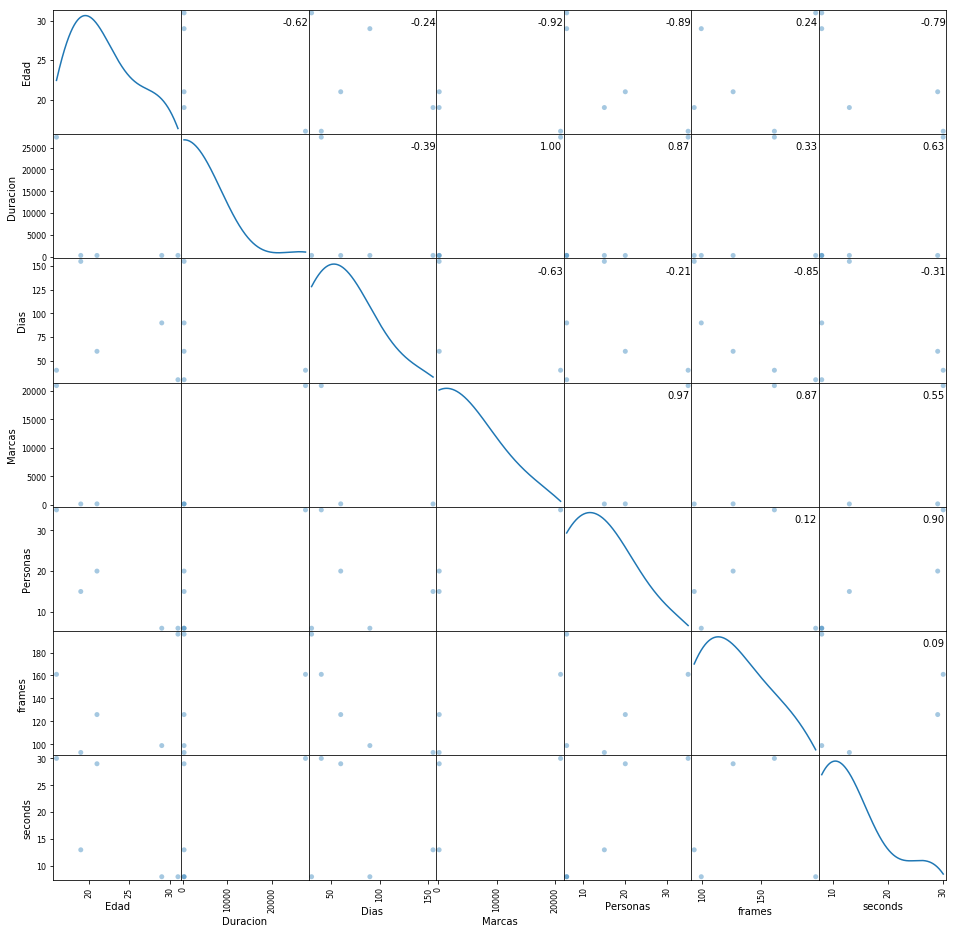
\includegraphics[width=\textwidth]{23}
\caption{}
\end{subfigure}
\caption{Resultados de los métodos de aprendizaje maquina}\label{fig:OpenCV}
\end{figure}

En la Figura \ref{fig:OpenCV}, se puede ver la correlación entre los parámetros evaluados para poder determinar los cambios de escena en los vídeos ganadores del SmartFilms.


\section*{Conclusiones}
La información proporcionada que se proceso fue insuficiente. Contábamos con aproximadamente 4600 registros de los cuales solo el 10\% tenía la información completa. Debido a que fue el primer año en registrarse el año 2015 fue el cuello de botella para procesar el resto de la información. El año 2016, se tuvo mayor participación en las categorías infantil y juvenil. En el año 2017, la cantidad de participantes extranjeros aumentó. En 2018, debido a que se contemplaron los dos festivales, el Colombiano y el Mexicano, la cantidad de extranjeros que participaron disminuyó, porque se decidió iniciar un festival nuevo en el país que más extranjeros aportaba al festival.

Se deberían agregar limitaciones a los campos de categoría de este festival, como los géneros de los filmes, las marcas de celulares y limitar la sinopsis a una cantidad precisa de caracteres. 


\subsection*{Agradecimientos}
Agradezco al Consejo Nacional de Ciencia y Tecnología (CONACYT) por haberme financiado una beca sin la cual no podría haber analizado estos datos.

Agradezco a Juan Beltrán, director creativo de Valencia Producciones y al festival SmartFilms, por haber proporcionado los datos para su análisis.

\section*{Referencias}
\bibliographystyle{plainnat}

\bibliography{mybiblio}


\section*{Anexo A} \label{AnexoA}

\begin{figure}[H]
\centering
\begin{subfigure}[t]{0.5\textwidth}
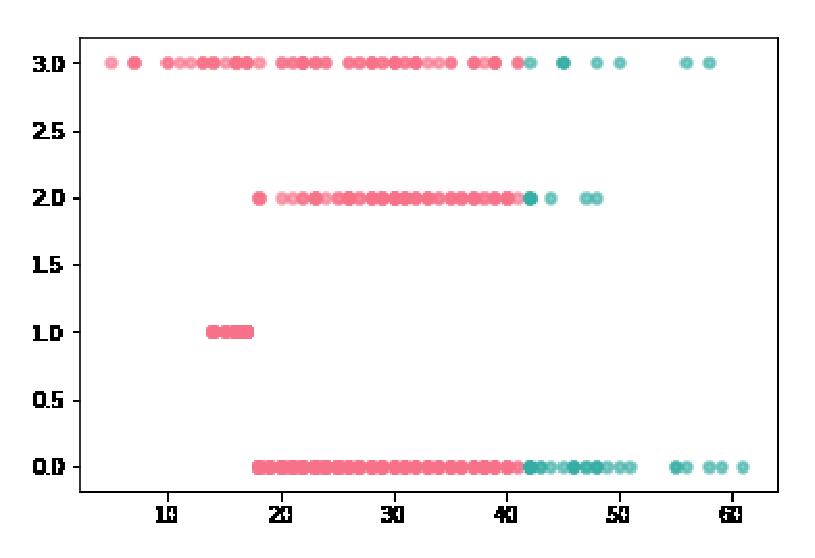
\includegraphics[width=\textwidth]{07}
\caption{}
\end{subfigure}

\begin{subfigure}[t]{0.5\textwidth}
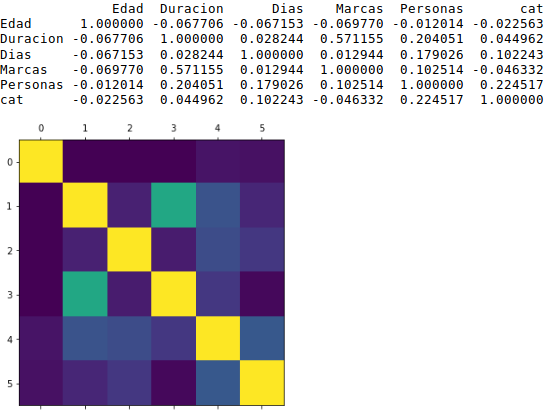
\includegraphics[width=\textwidth]{08}
\caption{}
\end{subfigure}

\caption{Modelos de regresion lineal múltiples}\label{fig:MRLMA}
\end{figure}


\section*{Anexo B}\label{AnexoB}

\begin{figure}[H]
\centering
\begin{subfigure}[t]{0.3\textwidth}
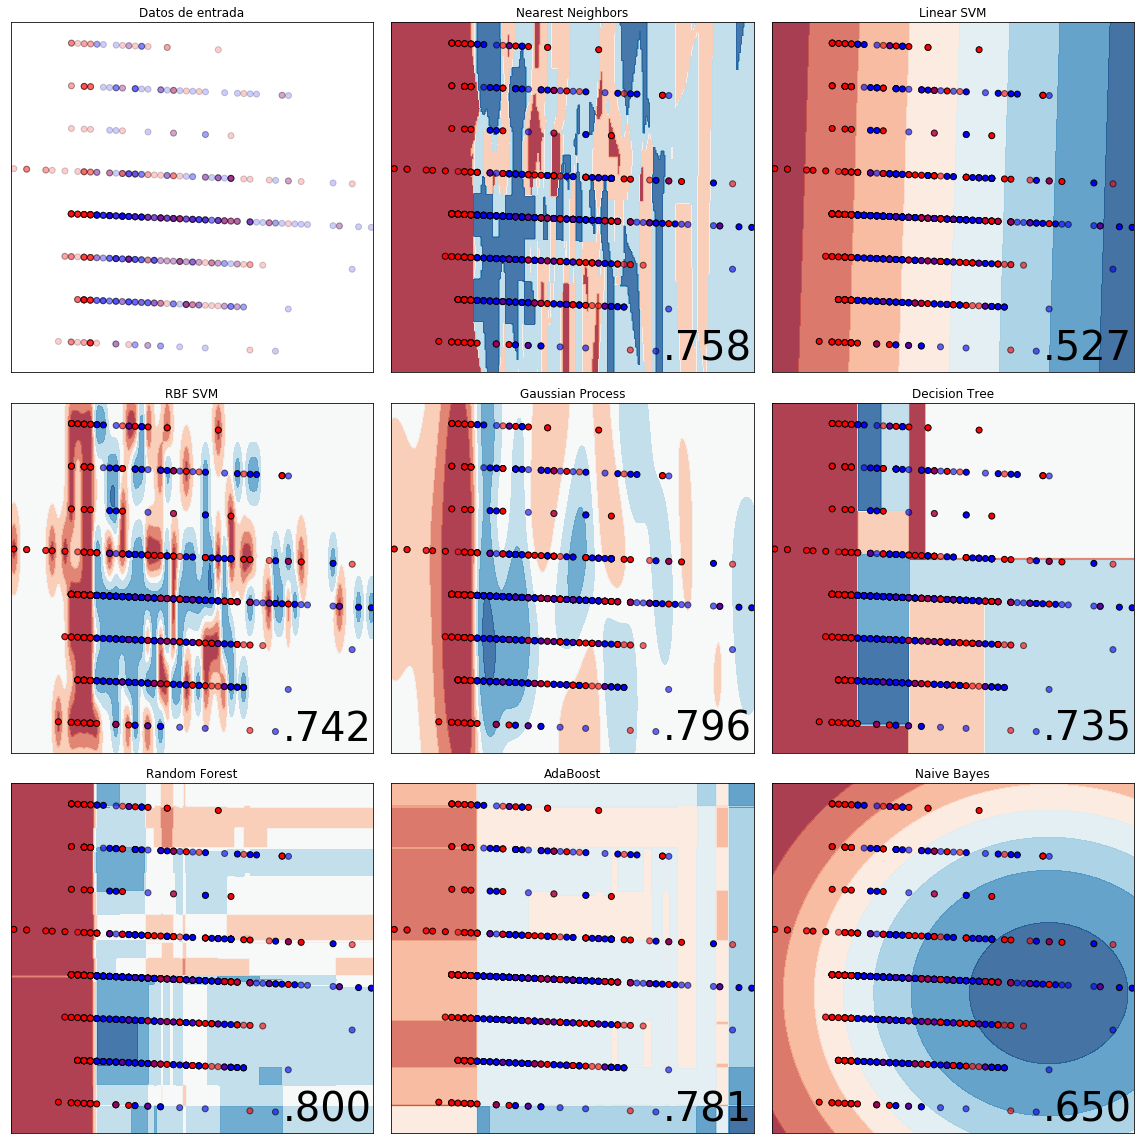
\includegraphics[width=\textwidth]{10}
\caption{}
\end{subfigure}

\begin{subfigure}[t]{0.3\textwidth}
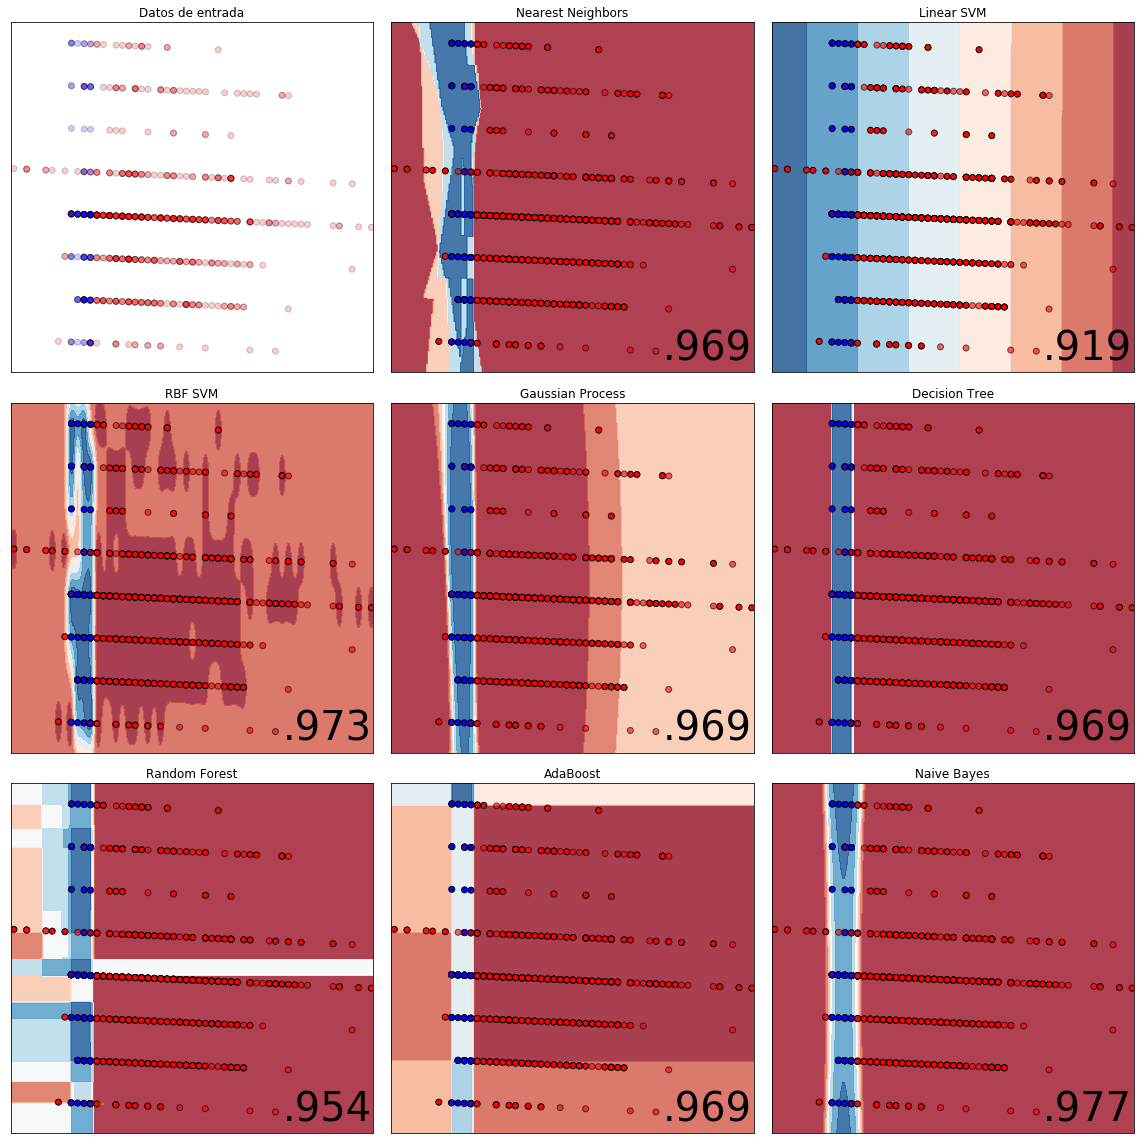
\includegraphics[width=\textwidth]{11}
\caption{}
\end{subfigure}

\begin{subfigure}[t]{0.3\textwidth}
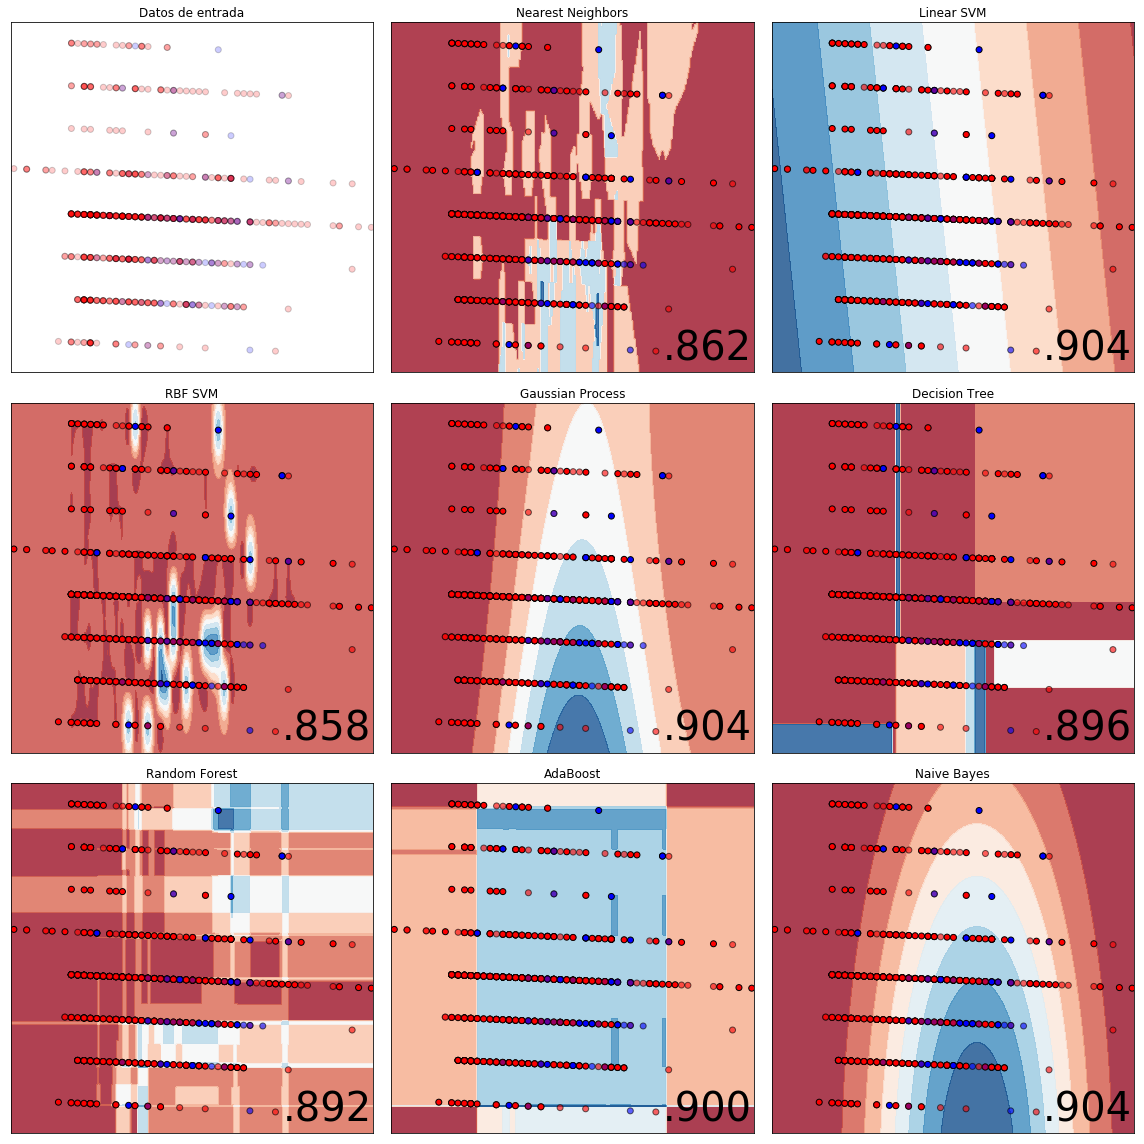
\includegraphics[width=\textwidth]{12}
\caption{}
\end{subfigure}

\begin{subfigure}[t]{0.3\textwidth}
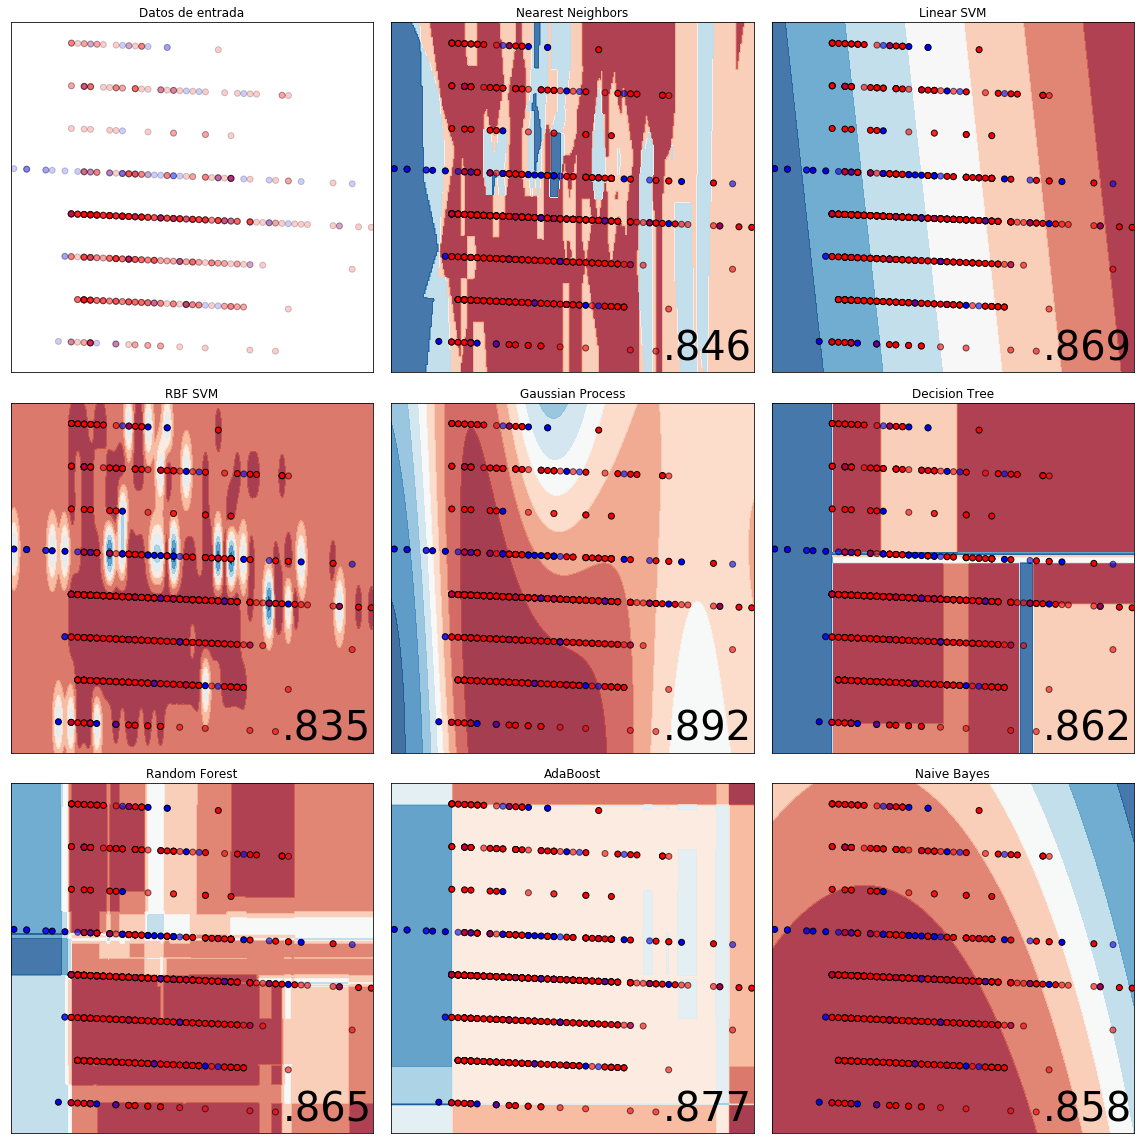
\includegraphics[width=\textwidth]{13}
\caption{}
\end{subfigure}
\caption{Gráficos de los métodos de aprendizaje maquina}\label{fig:MachineLearningGA}
\end{figure}

\end{document}